\section{Opis implementacji}
Aplikacja została napisana przy użyciu języków programowania bazujących na maszynie wirtualnej javy:
\begin{enumerate}
  \item Kotlin - podstawowy język użtyty do implementacji (prawie 90\% projektu)
  \item Java 8 - język użyty do generowania statystyk wykonania algorytmów
  \item JavaFX - technologia zastosowana do stworzenia graficzego interfejsu użytkownika (wraz z CSS)
\end{enumerate}

Architektura aplikacji jest modułowa. Zostały wydzielone części odpowiedzialne za obliczenia matematyczne, implementacje algorytmów, zapis i odczyt plików CSV, generację statystyk, definicję modelu danych oraz moduł zawierający aplikację korzystająca z pozostałych pakietów (\hyperref[fig:arch]{rys.~\ref*{fig:arch}}).

\begin{figure}[h]
  \center
  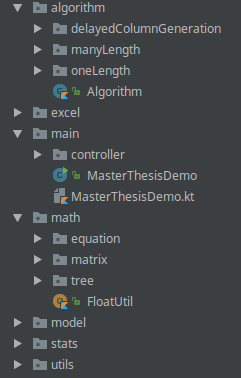
\includegraphics[scale=0.65]{../image/arch.png}
  \caption{Architektura aplikacji}
  \label{fig:arch}
\end{figure}

\begin{figure}[h]
  \center
  \includegraphics[scale=0.6]{../image/app_arch.png}
  \caption{Relacja między głównymi modułami aplikacji}
  \label{fig:app_arch}
\end{figure}

Architektura modułu odpowiedzialnego za implementację algorytmów posiada strukturę wzorca projektowego fasada. Klasy odpowiedzialne za konkretną implementację metody obliczenia rozkrojów rozszerzają klasę abstarkacyjną która definiuje wspólne funkcje oraz deklaruje metody które powinny zostać zdefiniowane w klasach potomnych. Główny moduł aplikacji wraz z modułem odpowiedzialnym za model danych tworzy implementację wzoraca Model-Widok-Kontroler (MVC). Klasa kontrolera zarządza widokiem stworzonym w języku FXML.

\hyperref[fig:java_arch]{Rynukek~\ref*{fig:app_arch}} opisuje korelację pomiędzy poszczególnymi modułami aplikacji wykorzystanymi do stworzenia programu z graficznym interfejsem użytkownika. Moduł Main odpowiedzialny jest za połączenie funkcjonalności aplikacji z GUI. Znajdują się w nim definicje widoku, wywołanie metod obliczających wynik z danych pobranych przez moduł excel oraz zapis rezultatu obliczeń. Moduł Model zawiera klasy odpowiedzialne za przechowywanie danych w aplikacji. Moduł Excel zawiera metody użyte do odczytu oraz zapisu danych w formacie CSV. Moduł Math zawiera operacje wykonywane na macierzach, jak również zawiera metodę do obliczania wartości nierówności metodą dwufazowej metody simplex, metodę podziału i ograniczeń do obliczenia wartości całkowitej z wyniku nierówności, metodę eliminacji Gaussa. W module tym znajduje się również klasa odpowiedzialna za tworzenie drzewa wykorzystanego przez metodę podizału i ogrniczeń. Moduł Algorithm zawiera klasy odpowiedzialne za obliecznie schematu rozkroju z wykorzystaniem metod brutalnej siły oraz opóźnionej generacji kolumn.

Rysunki \ref{fig:empty_win} oraz \ref{fig:fill_win} przedstawiają okno aplikacji, odpowiednio przed wypełnieniem danymi oraz po zakończeniu obliczeń.

Program posiada możliwość wczytania danych z pliku CSV, a następnie zapisanie danych wyjściowych również do pliku CSV lub TXT. Kolejnymi zaimplementowanymi funkcjonalnościami są:
\begin{enumerate}
  \item wyświetlenie danych wejściowych oaz wyniku w oknie aplikacji
  \item wybór algorytmu rozkroju
  \item dodanie wielu długości podstawowych z różnym kosztem - domyślnie koszt jest równy długości.
  \item wyświetlenie długości podstawowych w oknie aplikacji
  \item dodanie szerkości cięcia dla metody brutalnej siły
\end{enumerate}

\begin{figure}[h]
  \center
  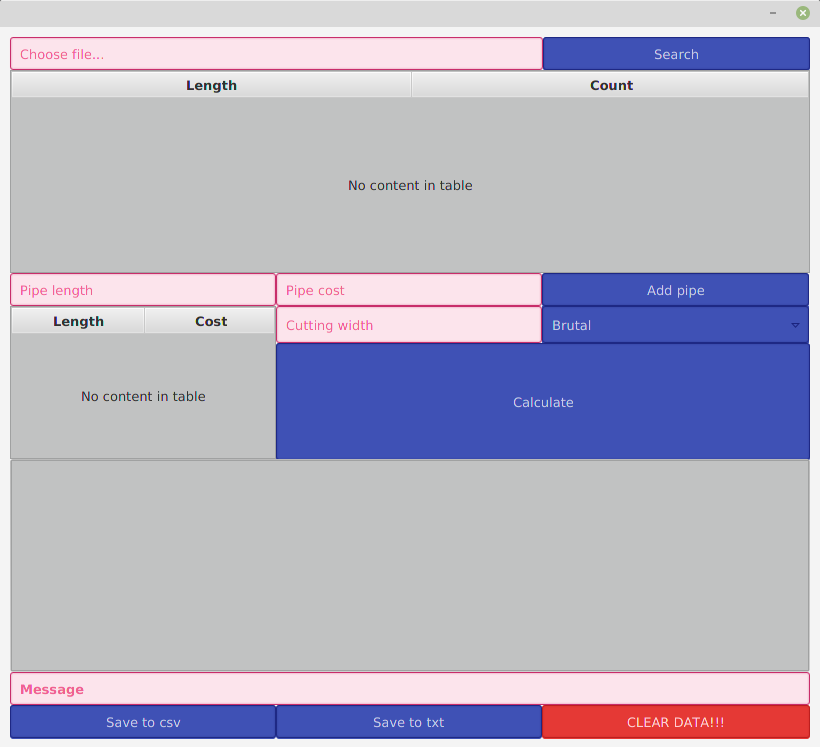
\includegraphics[scale=0.35]{../image/empty_win.png}
  \caption{Początkowe okno aplikacji}
  \label{fig:empty_win}
\end{figure}

\begin{figure}[H]
  \center
  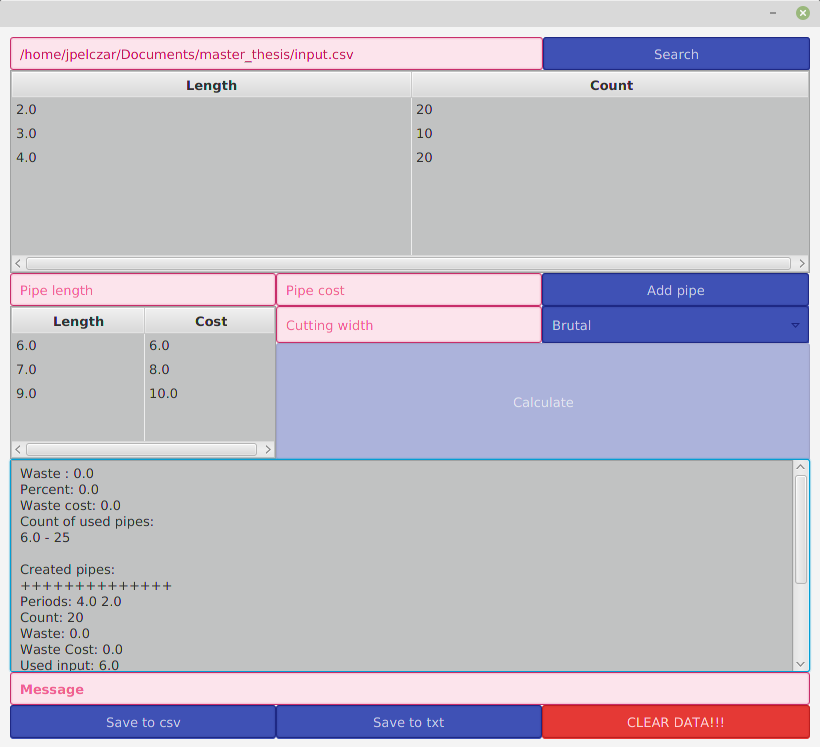
\includegraphics[scale=0.35]{../image/fill_win.png}
  \caption{Aplikacja po zakończonych obliczeniach}
  \label{fig:fill_win}
\end{figure}

\subsection{Java}
Język programowania Java jest jezykiem obiektowym z elementami programowania funkcyjnego wprowadzonymi od wersji 8. Aplikacje stworzone w tej technologii mogą być stosowane w różnych systemach operacyjnych, gdyż programy napisane w języku Java są kompilowane do plików class które umieszczane są w skompresowanej paczce jar. Pliki class następnie są przetwarzane przez maszynę wirtualną Javy (JVM - Java Virtual Machine) do postaci bytecode który jest wykonywany na urządzeniu. Istnieją implementacje JVM na większość używanych platform.

Tworzenie aplikacji w technologii Java jest możliwe poprzez użycie zestawu JDK (Java Development Kit). Uruchamianie tych aplikacji jest możliwe w środowisku JRE (Java Runtime Environment)  (\hyperref[fig:java_arch]{rys.~\ref*{fig:java_arch}}).

\begin{figure}[h]
  \center
  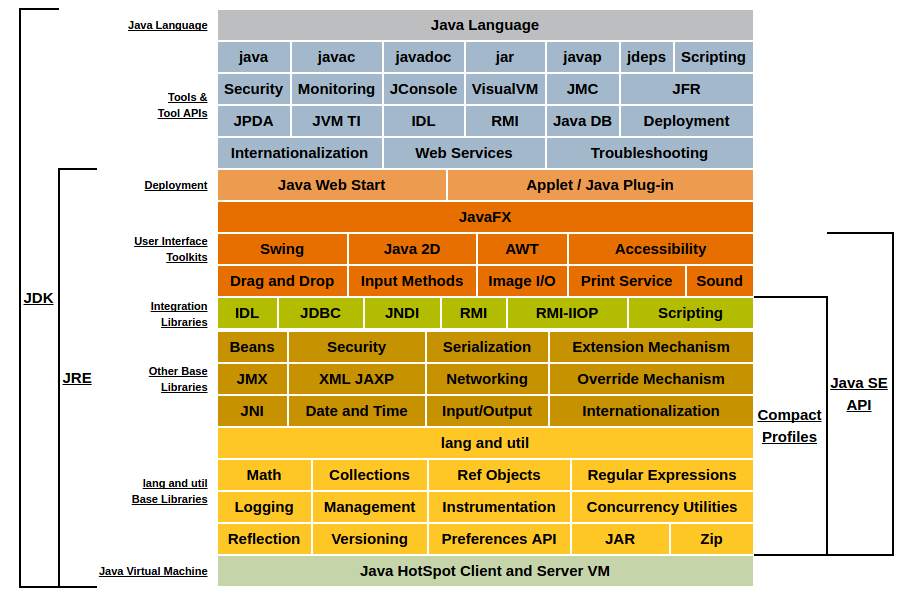
\includegraphics[scale=0.4]{../image/java_arch.png}
  \caption{Elementy składowe technologi Java \cite{OracleJavaArch}}
  \label{fig:java_arch}
\end{figure}

Podstawowym elementem technologii jest maszyna wirtualna. Jest to element technologii odpowiedzialny za niezależność programów od specyfikacji urządzenia oraz systemu operacyjnego. JVM jest abstarakcyjną maszyną obliczeniową. Podobnie jak rzeczywiste urządzenia posiada zestaw instrukcji pozwlających na sterowanie nią oraz wyonywanymi zadaniami. Maszyna wirtualna Javy nie zna języka Java, jedynie jego postać binarną zapisana w plikach class. Pliki te zawierają instrukcje dla JVM lub bytecode oraz inne wymagane informacje. Wiele języków programowania wykorzystuje tą cechę maszyny wirtualnej. Wymaganiem jest aby program był w postaci poprawnego pliku class, aby mógł zostać wykonany na maszynie wirtualniej.

Technologia Java zawiera ponadto zestaw podstawowaych bibliotek pozwlających między innymi na budowanie plików JAR, refleksję czyli dostęp do metod oraz pól klasy bez zachowania zasad bezpieczeństwa, zdalne wywoływanie metod (RMI) oraz tworzenie graficznego interfejsu użytkownika Swing oraz AWT. Środowisko deweloperskie jest rozszerzone o narzędzia potrzebne do stworzenia programu, przykładowo: javac - kompilator przetwarzający pliki java do plików class, javadoc - narzędzie do tworzenia dokumentacji oraz język opisu interfejsów IDL służacy do komunikacji międzyprocesowej.
\subsection{JavaFX}
Zgodnie z (\hyperref[fig:java_arch]{rysunkiem~\ref*{fig:java_arch}}), JavaFX jest częścią standardowego API technologi Javy. Jest to zestaw graficznych i multimedialnych pakietów które mogą zostać wykorzystane do stowrzenia graficznego interfejsu użytkownika spójnego na przestrzeni wszystkich systemów operacyjnych \cite{JavaFxInfo}. Głównymi cechami tej technologii są:
\begin{enumerate}
  \item Zgodność z językiem programowania Java oraz możliwość współpracy z innymi językami JVM, takimi jak Scala, Kotlin lub JRuby.
  \item Język FXML który jest językiem znaczników bazujący na języku XML. Jest on wykorzystywany do opisu graficznego interfesju użytkownika, podobnie jak HTML.
  \item WebView jest to technologia wykorzystująca WebKitHTML która umożliwia zagnieżdzanie stron internetowych w aplikacjach JavaFX. JavaScript uruchominy w widoku strony internetowej może wywoływać metody dostępne w języku Java. Od wersji JavaFX 8 możliwa jest również obsługa HTML5.
  \item Istniejące aplikacje Swing mogą zostać zaktualizowane o możliwości JavaFX takie jak odtwarzanie treści multimedialnych oraz wyświetlanie stron internetowych.
  \item Wbudowana obsługa kaskaowych arkuszów stylów oraz komponentów intefejsu użytkownika umożliwia tworzenie spersonalizowanych aplikacji pod względem wyglądu interfejsu użytkownika.
  \item Obsługa grafiki 3D została dodana w wersji 8 JavaFX. Obiekty trójwymiarowe mogą być wyświetlane na odpowiednich z scenach z zastosowanym światłem. Klasa Camera odpowiedzialna jest za rendering widoku.
  \item Obsługa Canvas API umożliwia bezpośrednie rysowanie po obiekcie sceny która zawiera jeden element graficzny.
  \item Aplikacja zbudowana z Java oraz JavaFX jest umieszczona w paczce która może zostać uruchomiana na każdym urządzeniu które obsługuje wirtualną maszynę Javy.
  \item Ponadto JavaFX umożliwia obsługę drukowania, wielopunktowego dotyku, wysokich rozdzielczości.
\end{enumerate}

  \begin{figure}[h]
    \center
    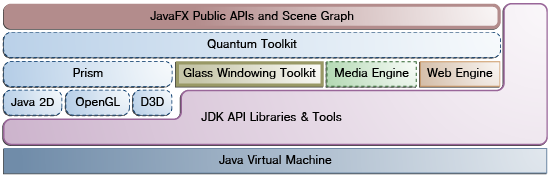
\includegraphics[scale=0.6]{../image/fx_arch.png}
    \caption{Architektura JavaFX}
    \label{fig:fx_arch}
  \end{figure}

\hyperref[fig:java_arch]{Rynukek~\ref*{fig:fx_arch}} opisuje architekturę technologi JavaFX. Zawiera ona zestaw deweloperski Java oraz maszynę wirtualną. Został również wyszczególniony silnik graficzny Prism odpowiedzialny za wyświetlanie widoków. Silnik ten może być wspomagany sprzętowo poprzez procesor graficzny. Na tym samym poziomie wraz z Prism znajduje się Glass Windowing Toolkik odpowiedzialny za współpracę z systmowymi oknami, zarządzaniu nimi oraz komunikację z systemowymi procesami odpowiedzlanymi za manipulację widokami. Prism, Glass Windowing Toolkit, silnik mutiledialny oraz internetowy współpracują ze sobą wykorzystując Quantum Toolkit który odpowiada za komunikację warstw powyżej z odpowiednimi elementami zarządzającymi grafiką.

\subsection{Kotlin}
Kotlin jest obiektowym językiem programowania który jest interpretowany do bytecode wywoływanego na maszynie wirtualnej Javy. Kotlin w porównaniu z Javą wnosi usprawnienia do programownaia proceduralnego. Kotlin jest zgodny z językiem Java, odnosi to skutek w możliwości łączenia obu języków programowania. Jest to technologia podobna do języka Scala jednak czas kompilacji został skrócony. Jest to język silnie rozwijający się w środowisku programistycznym Androida. Dopiero najnowsza wersja narzędzi deweloperskich Androida pozwala na wykorzystywanie niektórych elementów Javy 8. Kotlin zmniejsza liczbę nadmiarowego kodu potrzebnego do napisania przez programistę. Głównymi celami stworzenia technologii Kotlin były: pełna kompatybilność z językiem Java, zwiększenia bezpieczeństwa względem Javy (null safe), bardziej elastyczny oraz nieskomplikowany kod. Jedną z najciekawszych funkcjonalności języka Kotlin jest tworzenie metod rozszerzających daną klasę. Przykładowo może zostać zdefiniowana metoda $isNotEmpty()$ dla klasy $String$:
\lstset{language=Java}
\begin{lstlisting}[frame=single]
  fun String.isNotEmpty() = !this.isEmpty()
\end{lstlisting}
Metoda ta będzię dostępna dla każdego obiektu typu $String$ w programie.
